\documentclass[10pt,a4paper]{article}
\usepackage[utf8x]{inputenc}
\usepackage{ucs}
\usepackage{amsmath}
\usepackage{amsfonts}
\usepackage{amssymb}
\usepackage{hyperref}
\usepackage{graphicx}

\author{Olaf Radicke}
\title{Dokumentation der Funktionsweise der OSR-Dracut-Module}


\begin{document}

\maketitle

\newpage 

\tableofcontents

\newpage 

\section{Gernerell}

Als erstes wird vom Kernel nach dem Booten ein kleiner Binär-Code von Dracut ausgeführt, der dann seinerseits die in dash geschriebene Dracut-Module ausführt. Das erste Modul das von Darcut startet wird ist das Modul 99base. Das Erste was das Modul tut ist, dafür zu sorgen das dass initramfs geladen hat. Das Script was dafür verantwortlich ist, ist die \texttt{init}-Datei. Diese kann angepasst werden. Empfohlen wird aber stat dessen die Hooks zu verwenden. Hooks sind Scrips die vor oder nach definierten Ereignissen ausgeführt werden. Diese Hooks werden in den Modulen in den Dateien \texttt{install} definiert.

\subsection{Verwendete Hooks}

Die in den Modulen verwendeten Hooks sind:
\begin{description}
 \item[cmdline] Ein sehr früher Zeitpunkt. Hier werden die Kerne-Parameter ausgewertet werden die dem Bootloader mitgegeben wurden (Sei es als GRUB-Konfiguration oder beim Booten). Hier werden z.B. die wichtigsten Environment-Variablen gesetzt. 
 \item[pre-pivot] Das ist der letzte Hook der ausgeführt wird, bevor  das richtige root-Verzeichnis ein gehangen wird. Also ein guter Zeitpunkt für etweilige Aufräumarbeiten.
 \item[emergency] Ein solcher Hook ist in der Dracut-Doku nicht dokumentiert.
 \end{description}

In einem Script \texttt{check} wird eine Funktion \texttt{check()} definiert. Das Scrip \texttt{check} sollte 0 (null) zurückgeben, wenn alle Bedingungen erfüllt sind. Wird ein anderer Wert zurückgegeben, wird das Modul nicht von Darcut geladen.

\subsection{Weitere Schlüsselworte (Methoden) von Dracut}

\begin{description}
 \item[inst\_simple] Mit dem Schlüsselwort \texttt{inst\_simple} werden Dateien in das initramfs kopiert/installiert.
 \item[dracut\_install] Mit dem Schlüsselwort \texttt{dracut\_install} werden Software-Pakete in die ramsf-Umgebung installiert bzw. zur Verfügung gestellt.
 \end{description}
 
\subsection{Verwendete Darcut-Lib-Komandos}

Die Dracut-lib (\texttt{/usr/share/dracut/modules.d/99base/dracut-lib.sh}) stellt verschiedene Methoden zur Verfühgung. Benutzt werden von OSR:

\begin{description}
 \item [getarg()] Gibt die benutzten Kernel-Parameter zurück.
 \item [die()] Schreibt eine Meldung in \texttt{/dev/kmsg}, gibt eine Meldung auf der Standartausgabe aus und beendet das Script mit Rückgabelwert 1.
\end{description}

\section{Modul 95osr-chroot}

[TEXT]

\section{Modul 95osr-cluster}

[TEXT]

\section{Modul 96osr}

\subsection{In Initramfs installierte Dateien}

\begin{itemize}
 \item \verb|<|moddir\verb|>| /issue nach /etc
 \item \verb|<|moddir\verb|>|/shinit.sh nach /sbin
 \item \verb|<|moddir\verb|>|/lib/boot-lib.sh nach /lib/osr
 \item \verb|<|moddir\verb|>|/lib/defaults.sh nach /lib/osr
 \item \verb|<|moddir\verb|>|/lib/repository-lib.sh nach /lib/osr
 \item \verb|<|moddir\verb|>|/lib/rootfs-lib.sh nach /lib/osr
 \item \verb|<|moddir\verb|>|/lib/shinit.sh nach /lib/osr
 \item \verb|<|moddir\verb|>|/lib/std-lib.sh nach /lib/osr
\end{itemize}

\subsection{Von Dracut zu installierende Software}

\begin{itemize}
 \item awk
 \item cut
 \item tr
 \item expr
 \item mkdir
 \item basename
\end{itemize}

expr könnte mit awk abgedeckt werden.

\subsection{Definierte Hooks}


\begin{description}

\item[setup-osrenv.sh] cmdline  99
\item[parse-nodeid.sh] cmdline  2
\item[parse-cdsl.sh] cmdline 99
\item[mount-cdsl.sh] pre-pivot 1
\item[write-xfiles.sh] pre-pivot 90
\item[emergencyenv.sh] emergency 1
\end{description}

\subsubsection{setup-osrenv.sh}
\begin{description}
\item[Hook:] cmdline
\item[Priorität:] 99
\end{description}

\begin{figure}[h!]
 \centering
 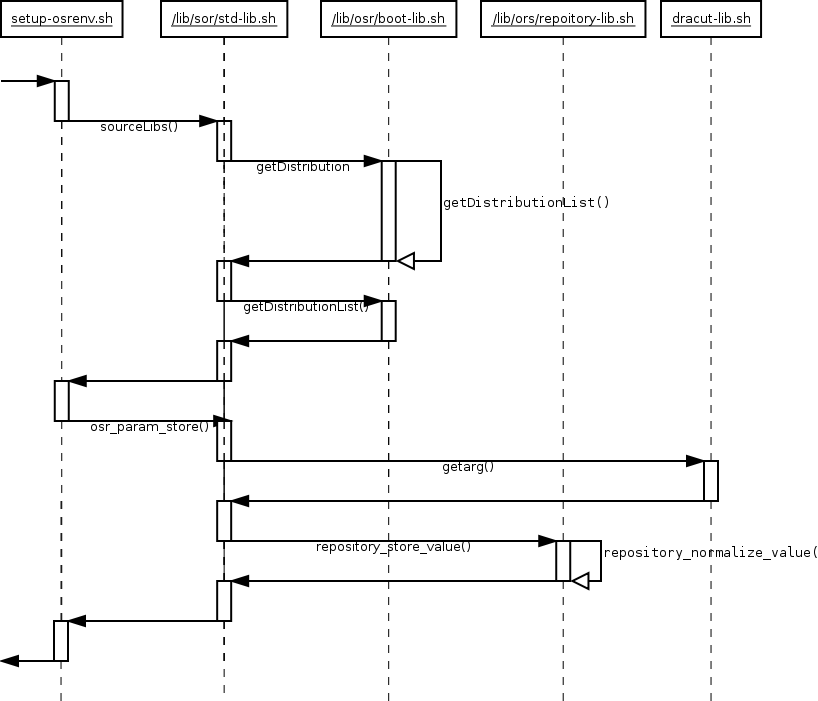
\includegraphics[scale=0.35]{./sequence_diagram_setup-osrenv_DE_de.png}
 \caption[]{Sequence-Diagram des setup-osrenv.sh-Scrips}
\end{figure}

Das Script lädt \texttt{dracut-lib.sh} und die \texttt{/osr/std-lib.sh}. Das Script versucht herauszufinden um welche Distribution es sich handelt. Und legt dann eine einfache Datenbank  mit Schlüssel-Werte-Paaren an. Die Schlüssel der gespeicherte Werte sind:

\begin{itemize}
 \item logofile
 \item shellrcfile
 \item shellissue
 \item shellissuetmp
 \item shell
 \item sysctlfile
 \item xtabfile
 \item xrootfsfile
 \item xkillallprocsfile
\end{itemize}


\subsubsection{parse-nodeid.sh}
\begin{description}
\item[Hook:] cmdline
\item[Priorität:] 2
\end{description}

\begin{figure}[h!]
 \centering
 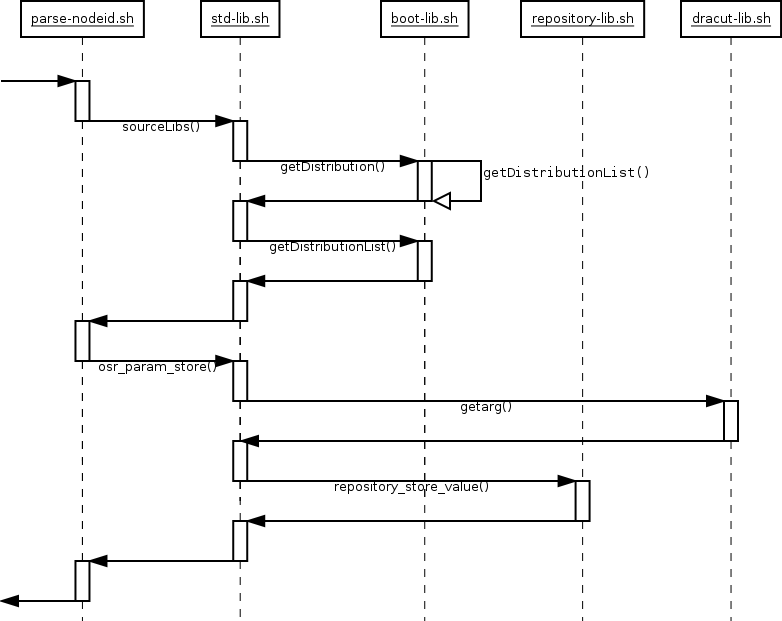
\includegraphics[scale=0.50]{./sequence_diagram_parse-nodeid_DE_de.png}
 \caption[]{Sequence-Diagram des parse-nodeid.sh-Scrips}
\end{figure}

Das Script überprüft noch ein mal die Art der Distribution und speichert den Namen in eine einfache Schlüssel-Werte-Tabelle (mittels der Funktion \texttt{repository\_store\_value()} aus der Datei  \texttt{repository-lib.sh})
Das Script überprüft ob den Kernel die Node-ID als Parameter übergeben wurde.


\subsubsection{parse-cdsl.sh}
\begin{description}
\item[Hook:] cmdline
\item[Priorität:] 99
\end{description}

Das Scrip legt in eine einfache Datenbank mit Schlüssel-Werte-Paaren an. Die Schlüssel der gespeicherte Werte sind:

\begin{itemize}
 \item cdsltree
 \item cdslsharedtree
 \item cdsllink
\end{itemize}

\subsubsection{mount-cdsl.sh}
\begin{description}
\item[Hook:] pre-pivot
\item[Priorität:] 1
\end{description}

\begin{figure}[h!]
 \centering
 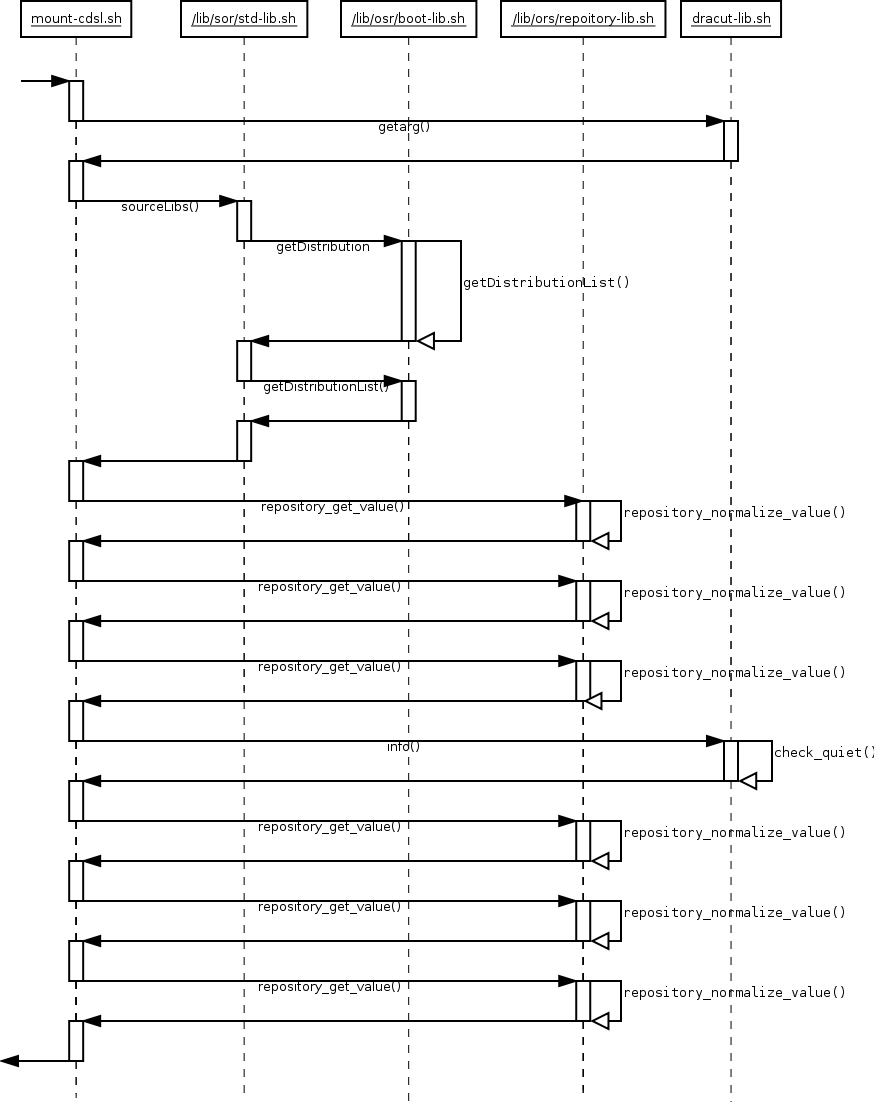
\includegraphics[scale=0.50]{./sequence_diagram_mount-cdsl_DE_de.png}
 \caption[]{Sequence-Diagram des mount-cdsl.sh-Script}
\end{figure}


\section{Modul 99osr-atix-legacy}

[TEXT]

\section{Quellen- und Literaturangaben}
\label{sec:quell}

\begin{itemize}
 \item fedora-Projekt: \url{http://fedoraproject.org/wiki/Dracut}
 \item Projektseite: \url{https://dracut.wiki.kernel.org/}
 \item News: \url{http://git.kernel.org/?p=boot/dracut/dracut.git;a=blob_plain;f=NEWS}
\end{itemize}





\end{document}